%!TEX program = lualatex
%-------------------------------------------------------------------------------
% 0Main.tex
% 
% Главный файл НИР
%
% Автор шаблона: Гордеев Иван
%-------------------------------------------------------------------------------

% \documentclass[a4paper, 14pt]{extarticle}  % Увеличить шрифт до 14 можно так
\documentclass[a4paper, 12pt]{article}

% TODO command to highlight
\newcommand\todo[1]{\textcolor{red}{#1}}  % использование: \todo{text}
\usepackage{tabularx}
%-------------------------------------------------------------------------------
% data.tex
% 
% Файл с основными сведениями для генерации титульника и мета информации
% определенные здесь команды можно использовать и в тексте.
% После замены на свои данные необходимо убрать команды \todo
%
% Автор шаблона: Гордеев Иван
%-------------------------------------------------------------------------------

%%% Основные сведения %%%
\newcommand{\UniversityFirst}{Государственное бюджетное образовательное учреждение высшего образования Название области}
\newcommand{\UniversitySecond}{<<Название университета>>}
\newcommand{\City}{Город}

\newcommand{\Year}{\the\year}

\newcommand{\male}{} % Раскомментировать если автор мужчина
% \newcommand{\female}{} % Раскомментировать если автор женщина

\newcommand{\AuthorFirst}{Иван}  % Имя автора
\newcommand{\AuthorSecond}{Иванов}  % Фамилия автора
\newcommand{\AuthorThird}{Иванович}  % Отчество автора
\newcommand{\AuthorInitials}{И.\,И.}  % Инициалы автора
\newcommand{\AuthorGroup}{0000}  % Номер группы автора

\newcommand{\SupervisorTitles}{нс Организации}  % Регалии научрука работы
\newcommand{\SupervisorFirst}{Иван}  % Имя научрука
\newcommand{\SupervisorSecond}{Иванович}  % Фамилия науч. рук.
\newcommand{\SupervisorThird}{Иванов}  % Отчество науч. рук.
\newcommand{\SupervisorInitials}{И.\,И.}  % Инициалы науч. рук.

\newcommand{\AuthorFaculty}{естественных и инженерных наук}  % Название факультета автора (без слова "Факультет")
\newcommand{\AuthorDepartment}{название}  % Название кафедры автора (без слова "Кафедра")

\newcommand{\Title}{Название НИР}  % Название НИР (Тема)
         % Основные сведения (здесь нужно изменить значения на свои)
\usepackage{referate}  % Стилевой файл со всеми настройками
% \MakePerPage{footnote}     % Нумерация начинается с каждой страницы заново
% \MakePerPage{footcite}     % Нумерация начинается с каждой страницы заново
%-------------------------------------------------------------------------------
\begin{document} 

%-------------------------------------------------------------------------------
% Выбрать нужный титульный лист
%-------------------------------------------------------------------------------
% 1-title.tex 
% 
% Файл титульного листа
%
% Автор шаблона: Гордеев Иван
%-------------------------------------------------------------------------------

\begin{center}

\begin{minipage}{12cm}
\begin{center}
\textbf{\UniversityFirst} \\[-0.1cm]
\end{center}
\end{minipage}

\textbf{\UniversitySecond} \\[-0.1cm]

\textbf{Факультет \AuthorFaculty} \\[-0.1cm]

Кафедра \AuthorDepartment \\[4.cm]

\large \textbf{ОТЧЕТ ПО ПРОИЗВОДСТВЕННОЙ ПРАКТИКЕ:} \\[0.1cm]

\textbf{Научно-исследовательская работа} \\[0.1cm]

\Title \\[4.cm]
\end{center} 

\hfill
\begin{minipage}{0.4\linewidth}
\begin{flushright}

\ifdefined\male
{
\small Выполнил: \\
студент группы \AuthorGroup \\
}
\else
{
\small Выполнила: \\
студентка группы \AuthorGroup \\
}
\fi

\AuthorSecond\ \AuthorFirst\ \AuthorThird \\
Руководитель: \\
\SupervisorTitles,\ \SupervisorSecond\ \SupervisorInitials \\

\rule{0.5\linewidth}{0.5pt}

Рекомендуемая оценка: \\

\rule{0.5\linewidth}{0.5pt}

\end{flushright}
\end{minipage}

\vfill
\begin{center} 
\small{г. \City,\ \Year\ г.}
\end{center} 

\thispagestyle{empty}
  % Титульный лист без логотипа
% %-------------------------------------------------------------------------------
% 1-title.tex 
% 
% Файл титульного листа
%
% Автор шаблона: Гордеев Иван
%-------------------------------------------------------------------------------

\begin{center}
\begin{minipage}{12cm}
\begin{center}
\textbf{\UniversityFirst} \\[-0.1cm]
\end{center}
\end{minipage}

\textbf{\UniversitySecond} \\[-0.1cm]

\textbf{Факультет \AuthorFaculty} \\[-0.1cm]

Кафедра \AuthorDepartment \\[1.cm]

\begin{figure}[H]
\flushright

\includegraphics[width=0.3\linewidth]{img/logo}
\captionsetup{labelformat=empty}
\caption{}
\label{img:Logo}
\end{figure}

\large \textbf{ОТЧЕТ ПО ПРОИЗВОДСТВЕННОЙ ПРАКТИКЕ:} \\[0.1cm]

\textbf{Научно-исследовательская работа} \\[0.1cm]

\Title \\[4.cm]
\end{center} 

\hfill
\begin{minipage}{0.4\linewidth}
\begin{flushright}

\ifdefined\male
{
\small Выполнил: \\
студент группы \AuthorGroup \\
}
\else
{
\small Выполнила: \\
студентка группы \AuthorGroup \\
}
\fi

\AuthorSecond\ \AuthorFirst\ \AuthorThird \\
Руководитель: \\
\SupervisorTitles,\ \SupervisorSecond\ \SupervisorInitials \\

\rule{0.5\linewidth}{0.5pt}

Рекомендуемая оценка: \\

\rule{0.5\linewidth}{0.5pt}

\end{flushright}
\end{minipage}

\vfill
\begin{center} 
\small{г. \City,\ \Year\ г.}
\end{center} 

\thispagestyle{empty}
  % Титульный лист с логотипом университета (img/logo.png)
%-------------------------------------------------------------------------------

\thispagestyle{empty}

\setcounter{figure}{0}  % Скинуть счетчик после лого на титульнике

\setstretch{1.}  % Изменить отступ для оглавления 
\tableofcontents
\setstretch{1.5}  % Далее в тексте должен быть полуторный отступ

\addtocontents{toc}{~\hfill\textbf{Стр.}\par}  % Добавить Стр. в содержании
\clearpage

%-------------------------------------------------------------------------------
% 2-intro.tex 
% 
% Файл главы с введением
%
% Автор шаблона: Гордеев Иван
%-------------------------------------------------------------------------------

\section*{\center Введение}
\addcontentsline{toc}{section}{Введение}

Здесь и далее приведено \todo{примерное содержание НИР}. Показана примерная структура НИР и использование основных \LaTeX команд для генерации рисунков, таблиц, формул и т.\,д. 

Рентгеновская установка предназначена для облучения клеточных культур в соответствии с задаваемыми значениями дозы и/или времени облучения. Проводится моделирование различных режимов работы установки с последующим сравнением полученных результатов с результатами эксперимента, проведенного с использованием радиохромных пленок.

Альтернативой прямым экспериментальным измерениям выступает моделирование методом Монте-Карло (МК), которое позволяет упростить процесс получения необходимых параметров без существенных потерь в точности. К МК программам относятся: MCNP~\cite{MCNPweb}, FLUKA~\cites{Ferrari2005,Boehlen2014}, PHITS~\cite{Sato2018}, GEANT4~\cite{Agostinelli2003}. 

В данной работе при помощи Монте-Карло кода FLUKA определяются значения поглощенной дозы и кермы, а также исследуется явление электронного равновесия. 

  % Введение

%-------------------------------------------------------------------------------
% 31-chapter-one-name.tex
%
% Литературный обзор 
%
% Автор шаблона: Гордеев Иван
%-------------------------------------------------------------------------------

\section{Литературный обзор}\label{ch:overview}

\subsection{Взаимодействие фотонов с веществом}

Фотонное излучение, проходя через вещество, частично или полностью передает ему свою энергию. Это  в основном происходит посредством 3 основных типов взаимодействий: фотоэффекта, эффекта Комптона и образования электрон-позитронных пар. На Рис.~\ref{img:mu} показаны линейные коэффициенты ослабления в зависимости от энергии для данных процессов.

\begin{figure}[h!]
	\center{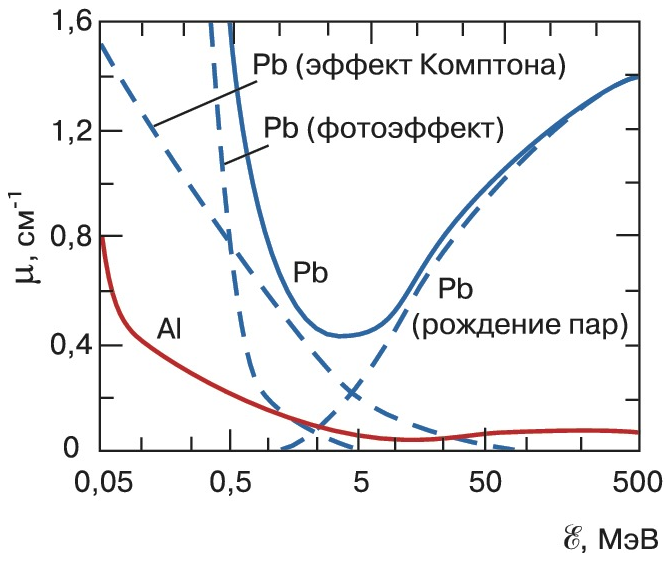
\includegraphics[scale=0.35]{img/mu}}
	\caption{Линейные коэффициенты ослабления для фотоэффекта, эффекта Комптона и образования электрон-позитронных пар от энергии \(\gamma\)-квантов}
	\label{img:mu}
\end{figure}

\subsubsection{Фотоэффект} 

Данный эффект заключается в поглощении атомом падающего на него фотона с энергией \(\varepsilon =\hbar\omega\) с последующим испусканием одного из связанных на \(i\)-й оболочке электронов. Из законов сохранения энергии и импульса следует, что фотоэффект не может происходить на свободном электроне. Фотоэффект возможен на любой электронной оболочке, однако электроны \(K\)-оболочки испускаются с большей вероятностью, по сравнению с более отдаленными от ядра оболочками.

Энергия вылетевшего электрона определяется как разность энергии налетающего фотона и энергии связи электрона \(i\)-ой оболочки с ядром:
\begin{equation}\label{eq:photo_eff}
E_e=\varepsilon-A
\end{equation}

\subsubsection{Эффект Комптона} 

Суть данного процесса заключается в изменении энергии фотона при его упругом столкновении с электроном. В результате соударения фотон теряет часть своей энергии и, как следствие, длина его волны увеличивается. Процесс происходит на свободных или слабосвязанных электронах в присутствии третьего тела для удовлетворения законов сохранения энергии и импульса. Изменение энергии фотона при эффекте Комптона описывается следующей формулой:

\begin{equation}\label{eq2}
E_{\gamma '}= \frac{E_{\gamma}}{1+(E_{\gamma}/m_ec^{2})(1-\cos\theta)},
\end{equation}

где \(E_{\gamma}\) "--- энергия падающего кванта, \(E_{\gamma '}\) -- энергия рассеянного кванта, \(\theta\) "--- угол рассеяния.

\subsubsection{Образование электрон-позитронной пары} 

Образование электрон-позитронной пары является результатом взаимодействия фотона с электромагнитным полем атома вблизи ядра. Данный процесс возможен только для тех фотонов, чья энергия превышает порог образования электрона и позитрона:

\begin{equation}\label{eq3}
	h\nu_\text{порог}=2m_0c^2=1.022 \ \text{МэВ}\ ,
\end{equation}
где \(\nu_\text{порог}\) "--- частота падающего фотона, \(m_0\) "--- масса покоя электрона.
  % Раздел 1

%-------------------------------------------------------------------------------
% 32-chapter-two.tex
%
% Материалы и методы исследования
%
% Автор шаблона: Гордеев Иван
%-------------------------------------------------------------------------------

\section{Материалы и методы исследования}
\label{ch:methods}

\subsection{Рентгеновская установка}

В данной работе интерес представляют дозиметрические характеристики излучения рентгеновской трубки установки CellRad (см. Рис.~\ref{img:CellRad}). Характеристики определялись путем моделирования. Основные параметры установки приведены в Таблице~\ref{tab:parameters}.

\begin{figure}[!htb]
\begin{minipage}{0.5\linewidth}
\center
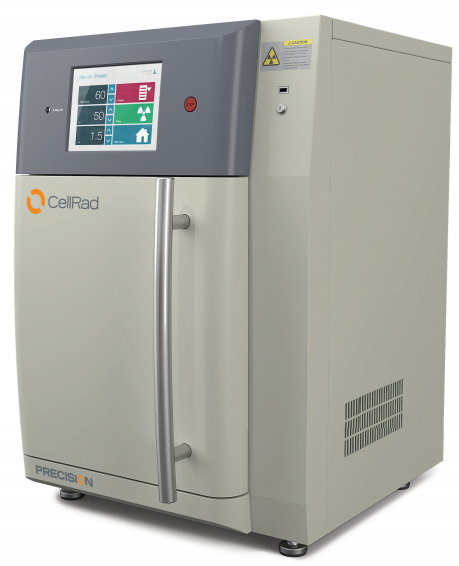
\includegraphics[width=0.9\linewidth]{img/CellRad}
\end{minipage}
% \hfill
\begin{minipage}{0.5\linewidth}
\center
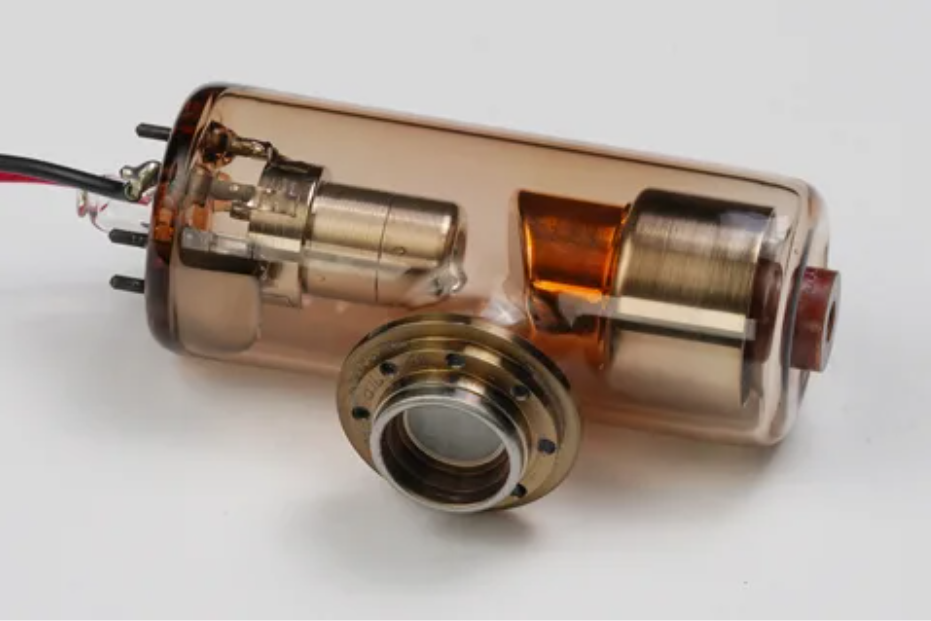
\includegraphics[width=1\linewidth]{img/XRayTube}
\end{minipage}
\vspace{5mm}
\caption{Установка CellRad фирмы Precision (слева), тип рентгеновской трубки (справа)}
\label{img:CellRad}
\end{figure}


\begin{table}[h]
\centering
\begin{tabular}{|c|c|c|c|}\hline
Макс. напряжение, кВ & Угол наклона анода, \textdegree  & Материал мишени & Внешняя фильтрация \\\hline
130 & 20 & W & 0.5 мм Al  \\\hline
\end{tabular}
\caption{Параметры рентгеновской трубки установки CellRad}
\label{tab:parameters}
\end{table}


Для расчета поглощенной дозы необходимо:
\begin{enumerate}[topsep=0pt,itemsep=-1ex,partopsep=1ex,parsep=1ex]
    \item Найти распределение флюенса по глубине проникновения в среду/материал. 
    \item Найти взвешенный по энергии флюенс.
    \item Найти значения массового коэффициента для всех соответствующих значений флюенса.
    \item Определить керму по формуле для каждого слоя.
    \item Определить глубину, на которой наблюдается электронное равновесие. С этой глубины можно считать, что поглощенная доза равна керме.
\end{enumerate} 
  % Раздел 2

%-------------------------------------------------------------------------------
% 33-chapter-two.tex
%
% Результаты
%
% Автор шаблона: Гордеев Иван
%-------------------------------------------------------------------------------

\section{Результаты}
\label{ch:results}

В данном разделе представлены результаты, которые заключаются в следующем ...
  % Раздел 3

%-------------------------------------------------------------------------------
% 4-conclusion.tex
% 
% Файл главы с заключением
%
% Автор шаблона: Гордеев Иван
%-------------------------------------------------------------------------------

\section*{\center Заключение}
\addcontentsline{toc}{section}{Заключение}

Изучена литература по физике взаимодействия $\gamma$-квантов с веществом. Освоена методика расчета дозиметрических величин на основе рентгеновского спектра в Монте-Карло программе транспорта ионизирующего излучения в веществе FLUKA. Изучено явление электронного равновесия, а также связь между поглощенной дозой излучения и кермой.

  % Заключение

%-------------------------------------------------------------------------------
% 5-biblio.tex
% 
% Файл отвечает за библиографию
% Для списка литературы используется biblatex-gost
% https://ctan.math.illinois.edu/macros/latex/contrib/biblatex-contrib/biblatex-gost/doc/biblatex-gost.pdf
%
% ВАЖНО, чтобы правильно оформлялись зарубежные источники на английском,
% нужно добавлять в английские источники
% hyphenation = {english},
% либо
% langid = {english},
% При компиляции могут выдаваться предупреждения о полях, которые движок не воспринимает
%
% Автор: Гордеев Иван
%-------------------------------------------------------------------------------

% \nocite{*}  % Отображает все источники из literature.bib, нужно убрать чтобы
% выводились только те, что используются в тексте
\printbibliography[heading=bibintoc]  % heading=bibintoc чтобы внести в оглавление
  % Список литературы

\end{document}
%-------------------------------------------------------------------------------
